


























































\subsection{Dark Matter Particle Physics}
\label{sec:dm_particle_physics}

% this paragraph should be shortened. It should state what dark matter is and then state the problem of the discrepancy of clear presence in astronomy but missing in particle physics and state that it is therefore one of the largest problems in physics. The next paragraph should merely give the reader an overview of the subsections in dark matter particle physics.

%\gls{dm} is an invisible and hypothetical form of matter motivated by astronomical studies that imply that \gls{dm} has a gravitational interaction with normal matter, i.e the matter that is included in the \gls{sm} of particle physics. Yet there are no experiments that have been able to detect \textit{\gls{dm} particles}, prove the creation of \gls{dm}, or prove a theory that explains \gls{dm} at the subatomic level. In cosmology \gls{dm} is a widely accepted explanation for observed gravitational effects of celestial bodies that cannot solely be explained by general relativity and normal matter. The bridge of \gls{dm} in cosmology to particle physics has not been trivial. By modern standards, however, this pressing discrepancy between \gls{dm}'s clear presence in cosmology and \gls{dm}'s absence in particle physics is perhaps the largest reason for why it is considered one of the largest unsolved problems in modern physics. \cite{bertone2016-history-dark-matter} \cite{cirelli2026-darkmatter} 

\Gls{dm} is the name given to a proposed form of invisible matter that does not
emit, absorb or scatter light. Astronomical and cosmological measurements reveal
gravitational effects that, within general relativity, cannot be explained by the
observed distribution of ordinary matter alone. Dark matter is the leading
explanation for these observations, but their cause has not been directly
established. In particular, no \gls{dm} particle or non-gravitational interaction
with the particles of the \gls{sm} has been confirmed in an experiment. This gap
between well-established astronomical observations and an unknown subatomic
explanation makes dark matter one of the largest unsolved problems in modern
physics \cite{bertone2016-history-dark-matter,cirelli2026-darkmatter}.


%\gls{dm} is the name given to an invisible matter that does not emit, absorb or scatter light, but whose gravitational influence is observed throughout the Universe.  Astronomical and cosmological measurements provide strong evidence %This line should not imply that it provides strong evidence for it, but rather dark matter is an explanation to explain observations of gravitational effects that cannot be referenced to normal matter for its presence,  yet no \gls{dm} particle or non-gravitational interaction with the particles of the \gls{sm} has been confirmed in an experiment. This gap between clear astronomical evidence and an unknown subatomic explanation makes dark matter one of the largest unsolved problems in modern physics \cite{bertone2016-history-dark-matter,cirelli2026-darkmatter}.



% UPDATE
%This subsection will give the reader a brief historical context to \gls{dm} and its introduction in particle physics, an introduction to the thermal freeze out framework that gives thermal relic \gls{dm}, and lastly a description of the Dark Bremsstrahlung particle interaction that is the basis for the \gls{ldmx}.

This subsection briefly traces the introduction of \gls{dm} into particle
physics before presenting thermal freeze-out, light dark matter and the dark
bremsstrahlung process that is the basis for the \gls{ldmx}.

\subsubsection{A Brief History of Dark Matter: from Astronomy to Particle Physics}
\label{sec:history}

%At the frontier of observation, a new tool can change what is visible. When Galileo Galilei (17th century) pointed the telescope at the sky, he measured that the movement of Jupiter had irregularities, implying 4 satellites of mass orbiting it, but the moons were invisible to the naked eye. These were not discoveries of \gls{dm}, but they illustrate two important ideas: nature may contain matter beyond the reach of ordinary perception, and a new instrument can move that reach \cite{bertone2016-history-dark-matter}. Just as the telescope did not create Galileo's moons, a reconstruction algorithm does not create new detector information either, it attempts to make better use of information that is already there.

At the frontier of observation, a new tool can change what is visible. When
Galileo Galilei pointed his telescope at the sky in the 17th century, he
resolved the faint glow of the Milky Way into stars and observed four
satellites in orbit around Jupiter, all previously invisible to the naked eye.
These were not discoveries of \gls{dm}, but they illustrate two important ideas:
nature may contain matter beyond the reach of ordinary perception, and a new
instrument can move that reach \cite{bertone2016-history-dark-matter}. Just as
the telescope did not create Galileo's moons, a reconstruction algorithm does
not create new detector information either, it attempts to make better use of
information that is already there.



\gls{dm} as a concept encapsulates this idea of matter that exists, but cannot
be perceived by ordinary means. The history of the physical phenomenon now
called dark matter, however, begins with measurements that revealed more
gravitating mass than astronomers could see. Astronomers could estimate the
visible mass of a galaxy or galaxy cluster from its light and independently
estimate the total mass required to explain how its stars or galaxies moved.
Several studies independently found that the visible mass was not enough. 
These studies included the recently rediscovered work by Lund University astronomer Knut Lundmark, whose
1930 comparison of the luminosities and mass estimates of five galaxies
preceded Fritz Zwicky's more famous 1933 study of the Coma cluster. Zwicky borrowed
the virial theorem from thermodynamics, modeling celestial bodies as particles, to show that the galaxies in Coma moved too rapidly for the
cluster to be held together by its visible mass alone.
Later measurements of galactic rotation curves showed a related
discrepancy: stars far from galactic centres moved faster than expected from the
visible matter
\cite{lundmark1930-galaxy-masses,bertone2016-history-dark-matter,
orodruin2016-lundmark-darkmatter}. For these astronomers, however, ``dark
matter'' generally meant unseen astronomical material such as faint stars, cold
gas or other non-luminous bodies, not necessarily a new elementary particle.

The transition from unseen astronomical matter to particle physics was neither
immediate nor automatic. It required both new evidence and a change in
scientific culture. Half a century ago, cosmology was still regarded by many physicists as a ''fringe science'' with limited predictive
power and testability, and the two communities rarely contributed to each
other's fields \cite{bertone2016-history-dark-matter}.

As cosmology became a recognized quantitative science, measurements of primordial element
abundances and the cosmic microwave background showed that baryonic
matter could not provide all the required mass. Within the standard
cosmological model, baryonic matter, meaning ordinary matter composed primarily
of protons and neutrons, accounts for only about \(16\%\) of the total matter
in the Universe. The remaining \(84\%\) is attributed to dark matter
\cite{cirelli2026-darkmatter}. Studies of structure formation further indicate
that the dominant component must have moved slowly enough to behave as cold matter. These results helped transform dark matter from a problem of unseen
astronomical objects into a problem that could require new particle physics.

Modified-gravity explanations, which attempt to reproduce these observations
without introducing a new non-baryonic matter component, have also been
explored, but none has accounted for the full range of observations as
successfully as the dark matter framework
\cite{bertone2016-history-dark-matter,cirelli2026-darkmatter}. 
%Even so, the astronomical observations are still isolated to a phenomenon of gravity and they do not by themselves establish that its cause is a particle.

The \gls{sm} describes the known elementary particles and their strong, weak
and electromagnetic interactions, while gravity is disconnected described separately by
general relativity. No known \gls{sm} particle simultaneously has the
properties required to account for the observed cold dark matter. A particle
interpretation therefore points beyond the \gls{sm}, to possibly a \gls{dm} sector. 
%A particle interpretation of dark matter therefore requires physics beyond the \gls{sm}. 
A viable \gls{dm} particle
candidate must have three key properties:




% I have made this enumerate exactly how I want it I needed to make it easier to read. 
\begin{enumerate}
    \item \textbf{Mass.} A \gls{dm} particle candidate must have mass higher than zero, accounting for the invisible mass in the Universe, and it explains its gravitational influence.
    \item \textbf{Stability.} 
    Observations in the cosmic microwave background imply 
    the existence of \gls{dm} in the early Universe and it remains abundant today. It must therefore be stable, or at least have a lifetime long
    enough to survive until the present day.
    \item \textbf{Almost no interaction with the \gls{sm}.} Gravity is described separately from the \gls{sm}, but it is the only established interaction between \gls{dm} and ordinary matter. \textbf{\emph{If}} \gls{dm} has any additional interactions with \gls{sm} particles, they must be sufficiently weak to have escaped detection in previous experiments. In particular, any electromagnetic interaction must be extremely weak.
\end{enumerate}


\subsubsection{Thermal Relics and the Sub-GeV Frontier}
\label{sec:thermal_relic}


Possible dark matter candidates span an enormous range of masses.
Figure~\ref{fig:dm_candidate_range} gives a schematic overview of several
frequently discussed regions. In this thesis, \gls{ldm} refers to particle dark
matter below approximately the GeV mass scale. The range of greatest relevance to
\gls{ldmx} is roughly from MeV to GeV masses. 
%\gls{ldm} is not one specific particle model, it is a lower-mass region containing many possible candidates and interaction mechanisms
\cite{battaglieri2017-cosmic-visions,ldmx2025-overview}.

\begin{figure}[htbp]
    \centering
    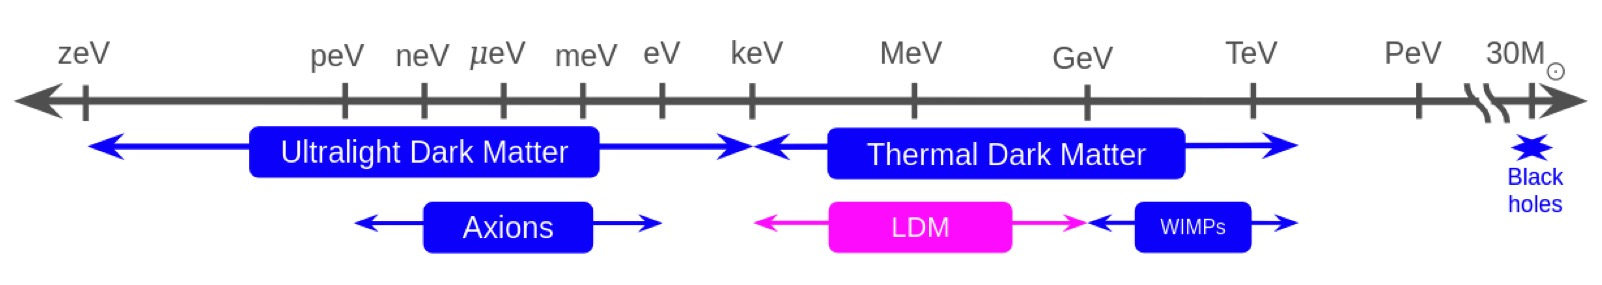
\includegraphics[width=\linewidth]{config/fig/dm_range.jpeg}
    \caption{Representative mass ranges for several \gls{dm} candidates and frameworks. The \gls{ldm} region relevant to LDMX is highlighted in magenta, while WIMP benchmarks occupy a higher-mass part of the broader thermal dark matter region. The boundaries are illustrative and model-dependent. Reproduced from Figure~4 of Ref.~\cite{gajdan2025-hcal-thesis}, which was inspired by Figure~1 of Ref.~\cite{battaglieri2017-cosmic-visions}.}
    \label{fig:dm_candidate_range}
\end{figure}

The \emph{thermal freeze-out} hypothesis is one possible explanation for the
amount of dark matter observed today. In this model one assumes that there exists an interaction
that connects the \gls{sm} and the dark sector. Given this assumption, in the hot and dense early Universe, particle collisions were frequent and energetic enough to create dark matter particles. Dark matter particles could also annihilate back into \gls{sm} particles. These reactions occurred rapidly enough to keep the two
sectors in \emph{thermal equilibrium}. 


As the Universe expanded, it became cooler and less dense. Creating massive
dark matter particles became increasingly difficult, while existing dark matter
particles continued to annihilate. Eventually, the particles became so dilute
that the annihilation rate fell below the expansion rate of the Universe.
Annihilation then became rare, and the number of dark matter particles in a
volume expanding with the Universe remained approximately constant. Their abundance had \emph{frozen out}, and the surviving population is called
a \emph{thermal relic}.

The surviving thermal relic depends on the strength of the interaction. A stronger
annihilation process remains effective for longer and leaves fewer dark matter
particles, while a weaker process causes an earlier freeze-out and leaves more
particles. For a specified particle model and mass, the observed dark matter
abundance therefore defines a target interaction strength
\cite{cirelli2026-darkmatter}. This is referred to as the \emph{thermal target}.
Thermal freeze-out does not define one universal dark matter mass range because
the result also depends on the particle model, its interactions and the history
of the early Universe.

The historically best-known thermal relic candidate is the \gls{wimp}. A
particle with a mass near the electroweak scale with a weak-strength interaction can freeze
out with approximately the observed abundance, a coincidence known as the
\emph{WIMP miracle}. Searches have strongly constrained many WIMP models
without finding a confirmed signal, although WIMPs as a class have not been
excluded. Experimental limits depend on both particle mass and interaction
strength. Below the GeV scale, the nuclear recoil produced by a dark matter
particle becomes difficult for traditional WIMP searches to detect, motivating
alternative searches for \gls{ldm}
\cite{cirelli2026-darkmatter,krnjaic2026-thermal-dark-photon,
ldmx2025-overview}.



\begin{figure}[htbp]
    \begin{minipage}[t]{0.48\linewidth}
        \centering
        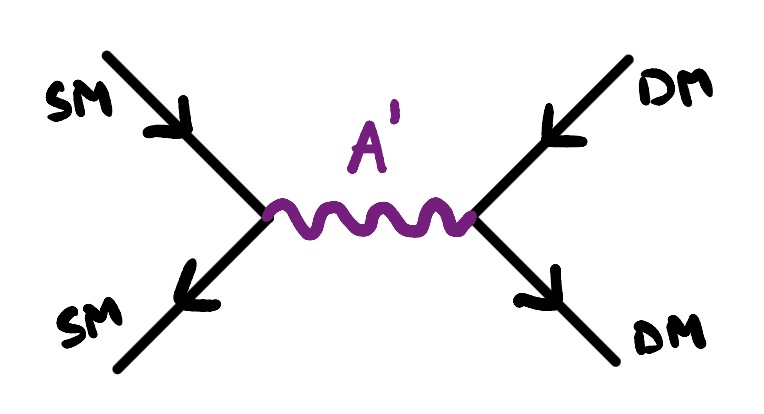
\includegraphics[width=\linewidth]{config/fig/dark_photon_feynman.jpg}
        \caption{Feynman diagram of conversion of a pair of \gls{sm} particles into a
        pair of \gls{dm} particles, mediated by a dark photon \(A'\).}
        \label{fig:sm_dm_dark_photon}
    \end{minipage}
    \hfill
    \begin{minipage}[t]{0.48\linewidth}
        \centering
        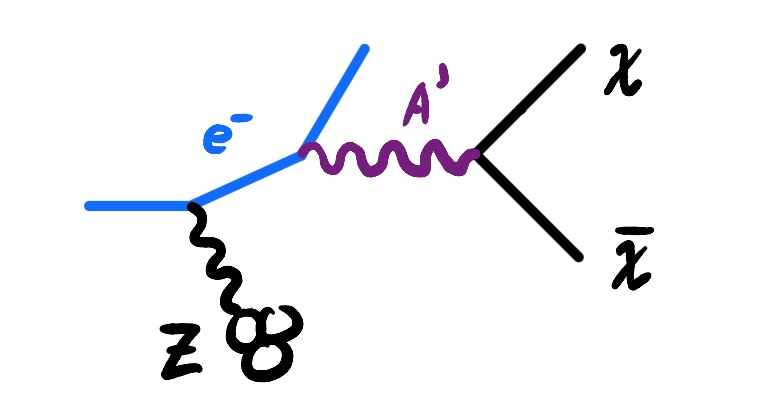
\includegraphics[width=\linewidth]{config/fig/dark_bremsstrahlung_feynman.jpg}
        \caption{Feynman diagram-sketch of dark bremsstrahlung.
        %in electron-nucleus scattering.
        The electron scatters and radiates a dark photon \(A'\), which decays into
        an invisible dark matter particle-antiparticle pair \(\chi\bar{\chi}\). The
        recoiling electron provides a visible signature by the law of conservation of momentum. Inspired by Ref.~\cite{helgstrand2025veto_power}.}
        \label{fig:dark_bremsstrahlung_feynman}
    \end{minipage}
\end{figure}

One way to connect \gls{ldm} to the \gls{sm} introduces
a new dark-sector gauge-boson mediator called the \gls{dark photon}, denoted by \(A'\) in
Figure~\ref{fig:sm_dm_dark_photon}. It can be
thought of as a dark-sector relative of the ordinary photon. A small kinetic mixing with the ordinary
photon allows the dark photon to interact weakly with electrically charged
\gls{sm} particles. In the invisible dark photon benchmark considered here, the dark
photon decays into a pair of dark matter particles, denoted by
\(\chi\bar{\chi}\)
\cite{cirelli2026-darkmatter,ldmx2025-overview}.


%An incoming electron scatters in the field of a target nucleus and radiates a dark photon, which decays into \(\chi\bar{\chi}\). The dark matter particles leave no measurable detector signal, but their production can instead be inferred from the imbalance between the incoming electron momentum and the reconstructed visible final state.


In an electron fixed-target experiment, the benchmark production reaction is
\emph{dark bremsstrahlung}, illustrated in
Figure~\ref{fig:dark_bremsstrahlung_feynman}. It is a dark-sector version of
ordinary bremsstrahlung. An incoming electron scatters in the field of a target
nucleus and radiates a dark photon, which then decays into
\(\chi\bar{\chi}\). The dark matter particles leave no measurable detector
signal. Their production can instead be inferred from the imbalance between
the incoming electron momentum and the reconstructed visible final state.
Unexplored thermal targets motivate the missing-momentum search for which
\gls{ldmx} is designed
\cite{akesson2018-ldmx,ldmx2025-overview}.

Dark bremsstrahlung turns the original astronomical question into a tangible
experimental one: can missing momentum reveal an invisible final state after
ordinary sources of imbalance have been rejected? The next subsection
introduces the detector built to answer that question.





\subsection{The Light Dark Matter eXperiment}
\label{sec:ldmx}

\subsubsection{Search Strategy and Physics Goal}
% This section is good in what it achieves and what it wants to tell, but the parts preceding this has been rewritten since and now there is dual information this section does not have to explain stuff again that was explained in previous section. An overview and review of this part with previous parts in mind is necessary. 

% I think this section is missing the perspective of what researches and collaborators are involved in this. It is cool to mention in one sentence in the first paragraph that it is planned in california the us but collaborators are also in other places of the world. 

% I think it would be suitable to explain the choice of tungsten, why tungsten materials? Bremsstrahluhn is implied to be relevant and to occur with tungsten, that could be explicitly stated in 1 sentence with very short explanation.

%Dark bremsstrahlung provides the main benchmark production process for the \gls{ldmx}. LDMX is an electron fixed-target \gls{missing momentum experiment} designed to search for sub-GeV \gls{dm}. An \(8\,\mathrm{GeV}\) electron beam will strike a thin tungsten target at End Station A at \gls{slac}. The momentum of each incoming electron is compared with the measured momentum and energy in the final state. A large imbalance can indicate that an invisible particle carried momentum out of the detector \cite{ldmx2025-overview}.

\Gls{ldmx} is an electron fixed-target \textit{missing momentum} experiment
designed to search for sub-GeV \gls{dm} through the dark-bremsstrahlung
process introduced above. The experiment is planned for End Station A at
\gls{slac} in Stanford, California and is developed by an international collaboration
with institutions in the United States and Sweden. An \(8\,\mathrm{GeV}\)
electron beam will strike a thin tungsten target. Tungsten is used because
its high atomic number gives a large production rate for low-mass dark
photons and helps reduce nuclear backgrounds at the chosen target thickness
\cite{ldmx2025-overview}.






% The explanations here have been repeated from the previous dark matter chapter. We should not repeat stuff find a way new formulation that goes straight to the point instead and trusts that the reader has read the previous part or can just simply do so if one wants to. 
In the dark bremsstrahlung benchmark, the beam electron radiates a
\gls{dark photon}, denoted \(A'\). The mediator couples weakly to electrically
charged \gls{sm} particles and can decay into a pair of dark-sector particles,
denoted by \(\chi\). It therefore provides a possible bridge between the
\gls{sm} and a dark sector. The \gls{dm} particles do not produce a
measurable detector signal. LDMX instead tests the model by searching for the
recoil of the electron and the missing momentum left by their production
\cite{akesson2018-ldmx,ldmx2025-overview}.

In the benchmark process, a candidate event has three main features. The electron leaves the target
with less energy than it entered with, it receives a transverse (perpendicular to the beam direction)
momentum kick, and no other visible final-state particle accounts for the
lost momentum. The combination is important because ordinary
\gls{sm} interactions can mimic parts of this signature when a
visible particle escapes detection. The trackers therefore measure the
incoming and recoil-electron momenta, while the calorimeters test whether
additional visible activity explains the apparent missing momentum
\cite{akesson2018-ldmx,ldmx2025-overview}.

The planned beam structure delivers approximately 20 million filled buckets
per second, with an average of one to two electrons in each bucket. This
corresponds to roughly 20 to 40 million electrons reaching the target per
second during operation. The exposure, measured in \gls{eot}, is not a
universal event count required to reject a null hypothesis. Rather, increasing
the exposure increases sensitivity to rarer production processes and weaker
interactions. The attainable exposure also depends on running time, detector
performance, backgrounds and radiation tolerance. LDMX is designed for a
staged programme beginning around \(4\times10^{14}\) \gls{eot} and extending
towards exposures of order \(10^{16}\) \gls{eot}, with projected sensitivity
up to three orders of magnitude beyond earlier searches
\cite{ldmx2025-overview}.

Useful exposure depends not only on how many electrons are delivered, but
also on which events can be triggered, stored and reconstructed. The ability
to retain events containing several electrons can therefore improve the
practical physics reach. This connection is developed further in
Section~\ref{sec:formalism}.

\begin{figure}[H]
    \centering
    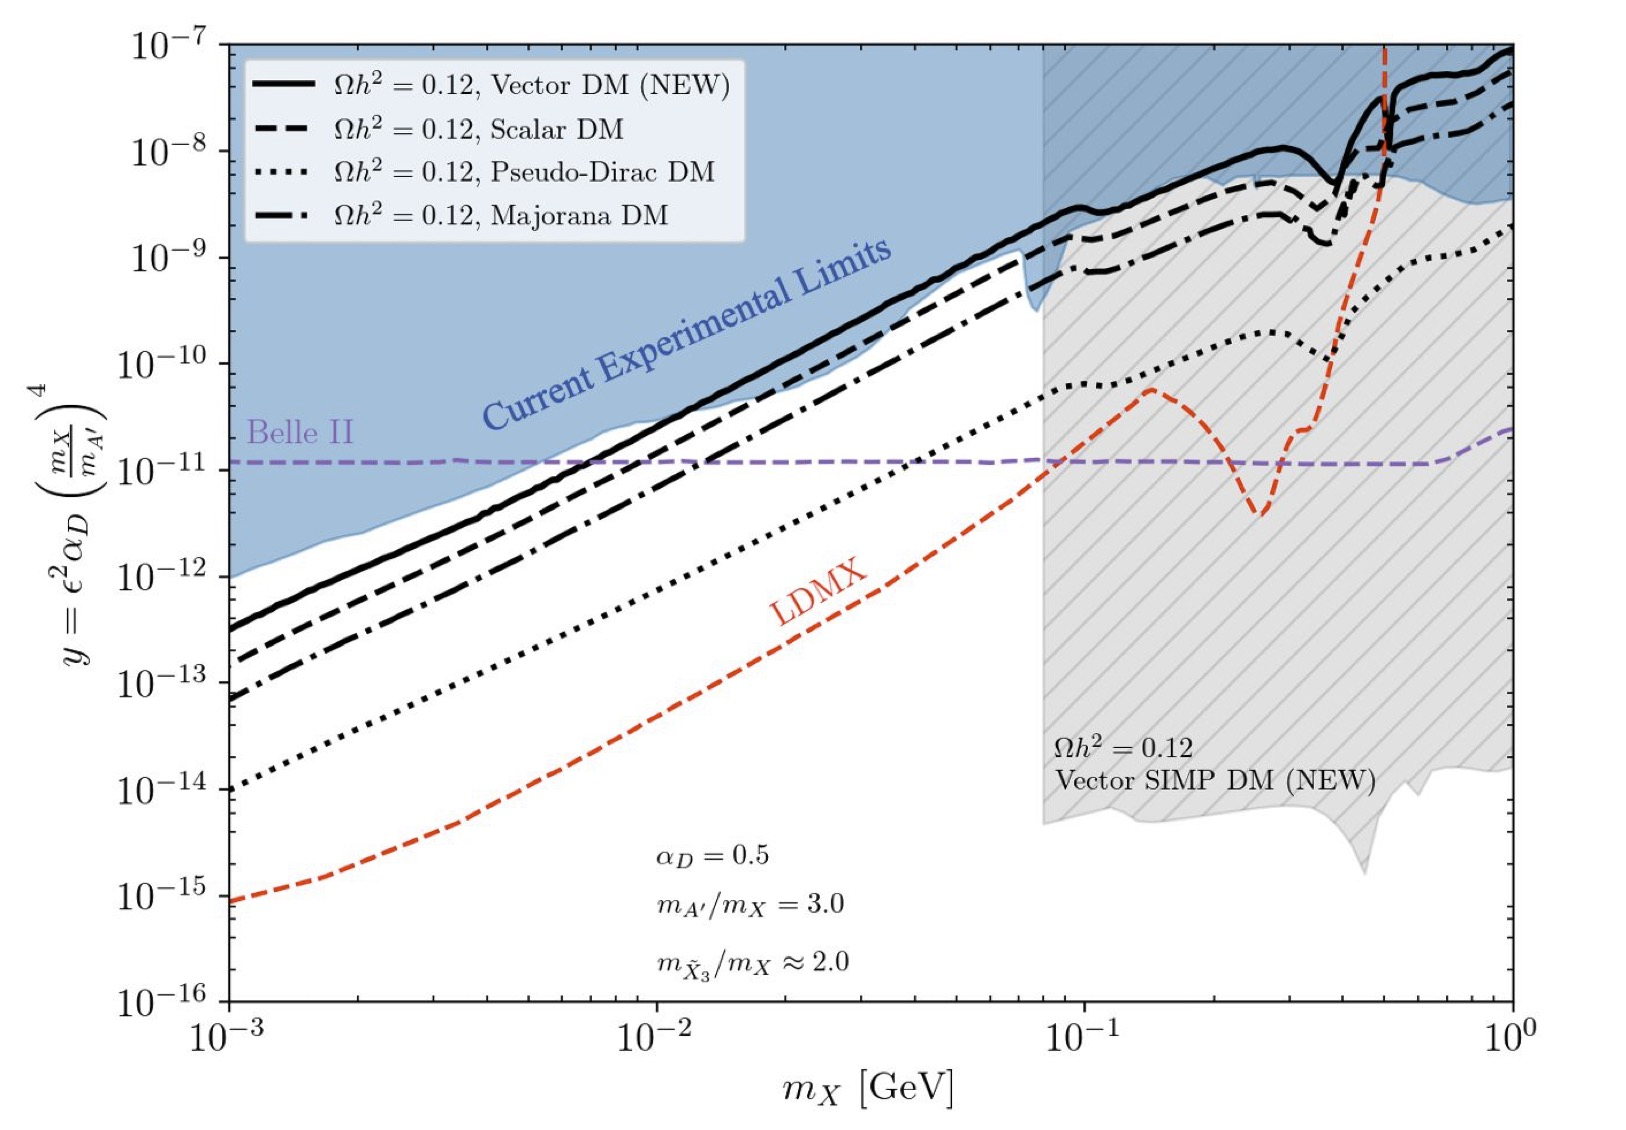
\includegraphics[width=0.80\linewidth]{config/fig/exclusion_ldmx.jpg}
    \caption{Representative comparison of thermal-relic targets with existing
    constraints and projected experimental sensitivity. The horizontal axis
    gives the dark-matter mass and the vertical axis gives the benchmark
    interaction quantity \(y\). Blue shows approximate existing constraints,
    purple shows the Belle~II projection, red shows the LDMX projection, and
    the black curves and grey region show several model-dependent \gls{dm} thermal
    targets. Reproduced from
    Refs.~\cite{catena2023-spin1-thermal-targets,ldmx2025-overview}.}
    \label{fig:exclusion_ldmx}
\end{figure}

Figure~\ref{fig:exclusion_ldmx} gives a representative view of the projected
reach. The horizontal axis shows the dark-matter mass, while the vertical
axis combines the assumed interaction strength and particle masses into the
benchmark quantity \(y\). The blue region represents parameter combinations
already constrained by earlier searches. The red curves show the smaller
interaction strengths that LDMX could test, thus expanding the frontier of 
search of \gls{dm}, while the black curves and grey
region show thermal-relic targets for several representative \gls{dm}
models. The figure is therefore a comparison within specified model
assumptions, not a model-independent exclusion of dark matter by mass alone
\cite{akesson2022-ldmx-status,catena2023-spin1-thermal-targets,
ldmx2025-overview}.

\subsubsection{Detector Layout}

Figure~\ref{fig:ldmx_detector_solid_model} shows the physical scale and
overall arrangement of the detector. The conceptual drawing in
Figure~\ref{fig:ldmx_beam_electron_schematic} illustrates the path of the
beam electron and the missing-momentum signature. The labelled cutaway in
Figure~\ref{fig:ldmx_detector_cutaway} shows the detector geometry along the
beam direction.

Two \gls{ts} modules are placed upstream of the silicon tagging tracker, and
a third is placed directly before the target. The tagging tracker measures
the incoming electron momentum. The electron then passes through the thin
tungsten target inside a dipole magnet. Its magnetic field bends charged
particles transversely according to their momentum, so a recoil electron
that has lost energy is deflected more strongly than an electron retaining
the full beam energy. A silicon recoil tracker downstream of the target
measures the momentum and direction of the outgoing charged particles.

The baseline target is \(0.1\) radiation lengths thick and has a transverse
size of \(4\,\mathrm{cm}\times10\,\mathrm{cm}\). Its small thickness limits
multiple scattering while retaining a useful production rate. The nominal
\(20\,\mathrm{mm}\times80\,\mathrm{mm}\) beam spot reduces peak detector
occupancy and helps to separate the showers from different electrons
\cite{ldmx2025-overview}.

The \gls{ecal} is placed behind the recoil tracker. It measures electrons,
photons and their shower shapes. The HCal surrounds the ECal at the sides
and rear. Its main role in the dark-matter search is to identify penetrating
hadrons and muons that could otherwise imitate missing momentum. Together,
the trackers and calorimeters measure the recoil electron and \emph{veto},
meaning reject, candidate events containing other visible particles. This
combined information distinguishes an invisible final state from ordinary
interactions in which visible particles were missed by one detector system
\cite{ldmx2025-overview}.

\begin{figure}[p]
    \centering

    \begin{minipage}[t]{0.48\linewidth}
        \vspace{0pt}
        \centering
        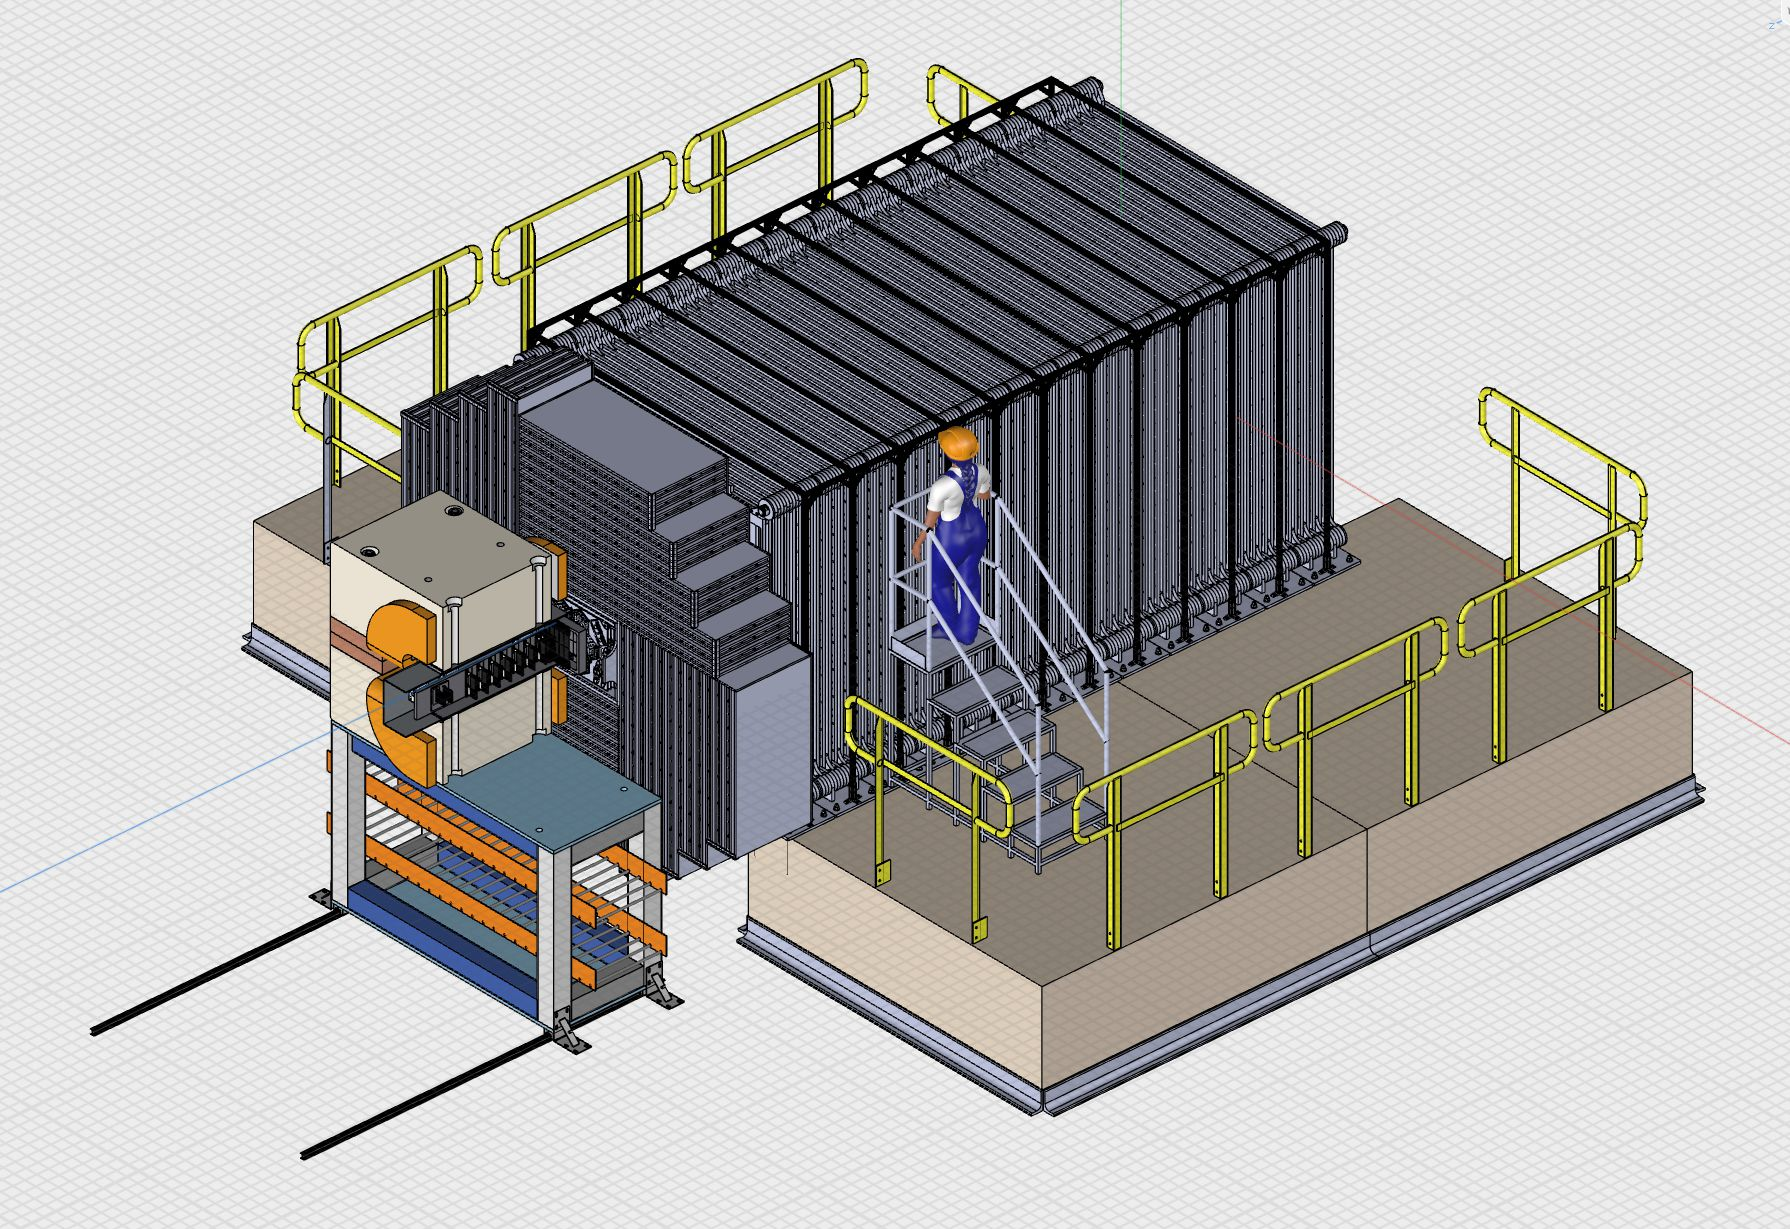
\includegraphics[
            width=\linewidth,
            height=0.20\textheight,
            keepaspectratio
        ]{config/fig/ldmx_detector_solid_model.jpg}
        \caption{Solid-model overview of the LDMX detector installation. The
        compact tracking and target region is located at the left, in front
        of the calorimeter systems. Sourced from Figure~3.1 of the 2025 LDMX
        design report \cite{ldmx2025-overview}.}
        \label{fig:ldmx_detector_solid_model}
    \end{minipage}
    \hfill
    \begin{minipage}[t]{0.48\linewidth}
        \vspace{0pt}
        \centering
        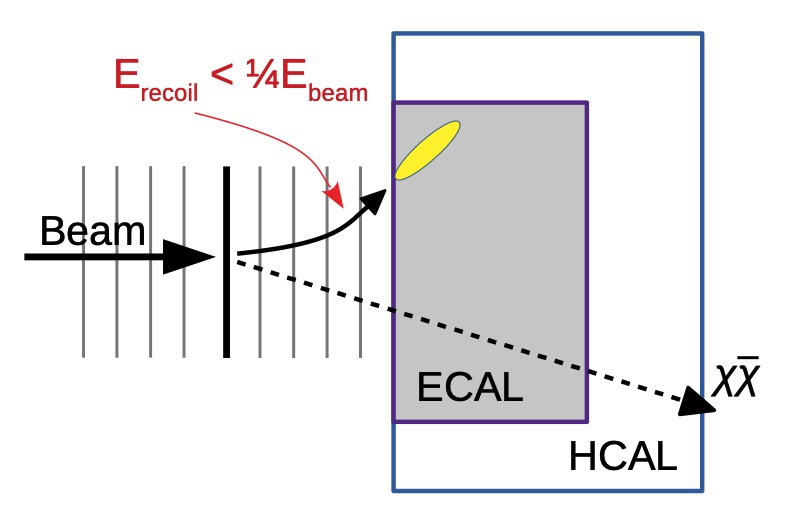
\includegraphics[
            width=\linewidth,
            height=0.20\textheight,
            keepaspectratio
        ]{config/fig/beam_electron_schematic.jpg}
        \caption{Conceptual illustration of the LDMX missing-momentum
        signature. After the beam electron passes through the tagging tracker
        and scatters in the thin tungsten target, a recoil electron carrying
        less than one quarter of the beam energy enters the ECal, while an
        invisible \(\chi\bar{\chi}\) pair carries away momentum. The ECal and
        HCal test for additional visible activity. Sourced from Figure~8 of
        the 2018 LDMX design report \cite{akesson2018-ldmx}.}
        \label{fig:ldmx_beam_electron_schematic}
    \end{minipage}

    \par\vspace{0.02\textheight}

    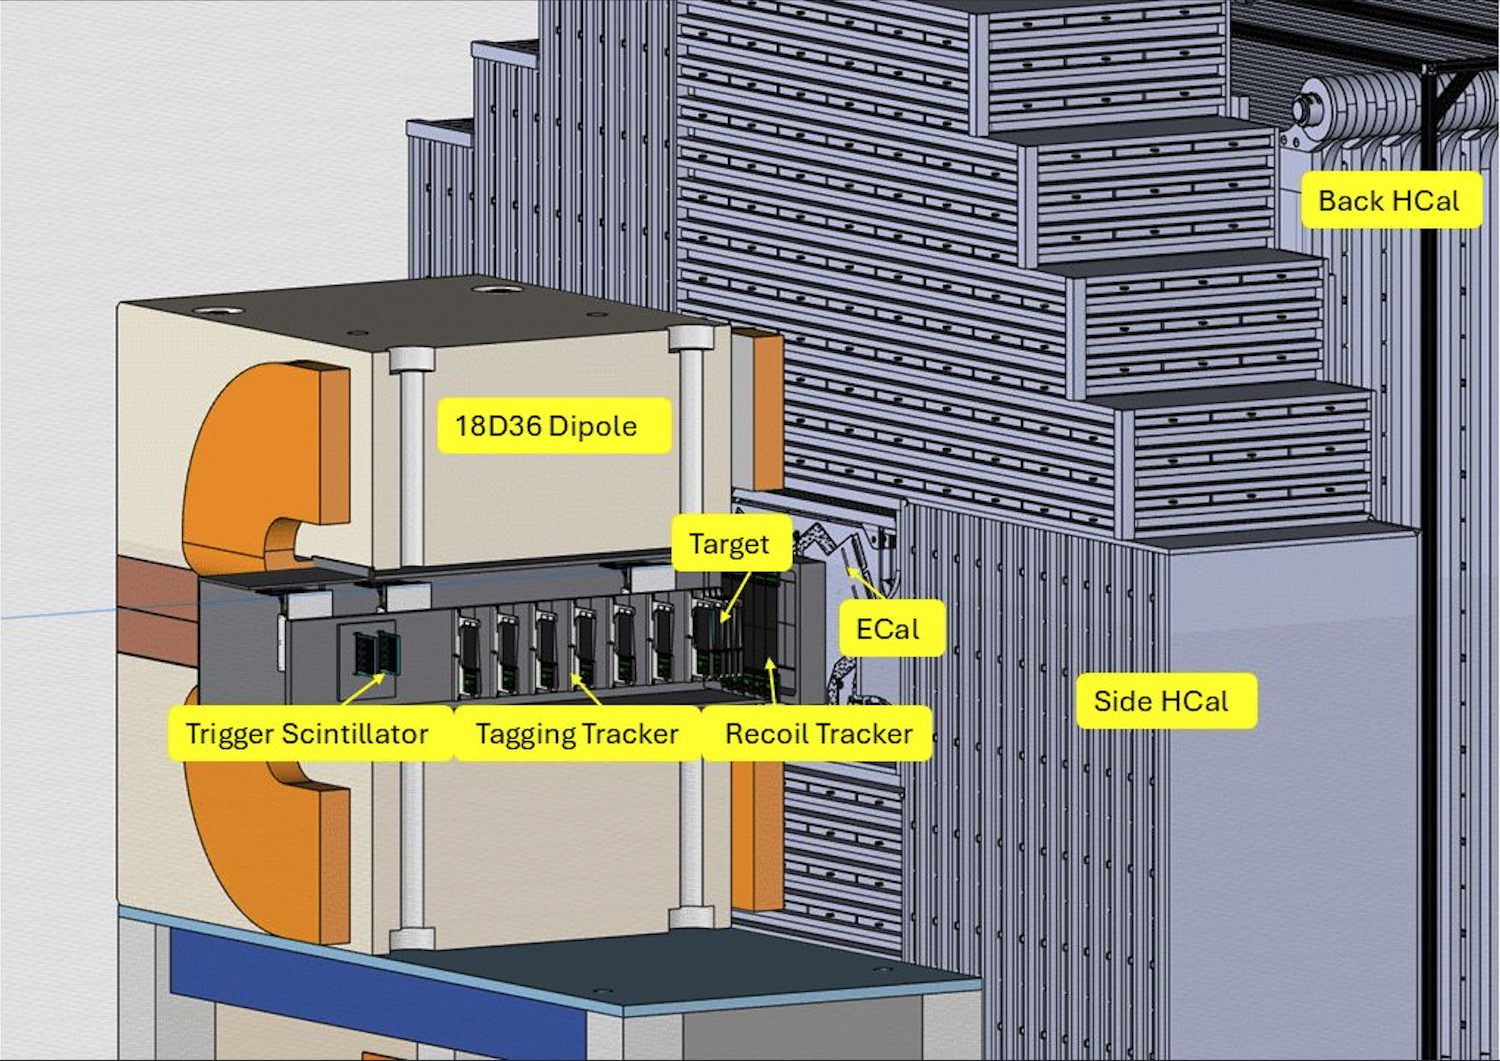
\includegraphics[
        width=\linewidth,
        height=0.47\textheight,
        keepaspectratio
    ]{config/fig/ldmx_detector_cutaway.jpg}
    \caption{Cutaway view of the LDMX detector. From left to right, it shows
    the Trigger Scintillator, tagging tracker, target inside the dipole
    magnet, recoil tracker, ECal, and the side and back HCal. Sourced from
    Figure~3.2 of the 2025 LDMX design report
    \cite{ldmx2025-overview}.}
    \label{fig:ldmx_detector_cutaway}
\end{figure}

\clearpage

\subsubsection{Electromagnetic Calorimeter and Electron Showers}

% The first section first sentence should be a 1 sentence summary what the main purpose or task with the ecal is. 
The main purpose of the \gls{ecal} is to measure the energy and spatial
development of electrons and photons, allowing the visible final state to be
reconstructed and backgrounds to be rejected. Its high-granularity 
silicon-tungsten design is a compact ''sibling detector'' of the \gls{hgcal} at the \gls{cms} experiment, from which LDMX adopts detector-module and readout technology
\cite{ldmx2025-overview}.


% This section should also mention that the ECal detector is a "sibling detector" since the design is based upon the CMS of CERN in one sentence, which a suitable reference if this info is not found in the design report. 
The ECal is a sampling calorimeter with a total depth of about \(40\)
radiation lengths. A radiation length \(X_0\) is the characteristic material
scale for energy loss by a high-energy electron through bremsstrahlung.
Tungsten layers initiate and develop electromagnetic showers, while
interleaved silicon layers sample their energy deposits. The final design
contains 32 silicon layers arranged as 16 bilayers, where each bilayer pairs
two silicon sampling planes around a common support and cooling structure.
The \path{ldmx-det-v15-8gev} geometry used in this thesis likewise produces
reconstructed ECal hits at 32 layer positions. The performance simulations in
the current (and newer) LDMX design report instead used an earlier geometry with 34
layers in 17 bilayers \cite{ldmx2025-overview}.

An energetic electron radiates photons through \gls{bremsstrahlung} as it
passes through tungsten. These photons can produce electron--positron pairs,
which radiate further photons. Repetition of these processes creates an
\gls{electron shower}. One incoming electron therefore produces energy
deposits in many cells and layers rather than a single detector hit. The energy contributions in the 3D pattern captures information about the electron position,
energy and shower development \cite{groom2024-passage-particles}.

The transverse size of an electromagnetic shower is commonly described by
the Molière radius \(R_{\mathrm{M}}\). For a homogeneous material, it is
calculated as
\begin{equation}
    R_{\mathrm{M}} = X_0\frac{E_{\mathrm{s}}}{E_{\mathrm{c}}},
    \qquad E_{\mathrm{s}} \simeq 21\,\mathrm{MeV},
    \label{eq:moliere_radius}
\end{equation}
where \(X_0\) is the radiation length, \(E_{\mathrm{s}}\) is a
material-independent scale energy, and \(E_{\mathrm{c}}\) is the critical
energy at which radiative and ionisation energy losses are comparable. On
average, about \(90\%\) of the shower energy is contained within a cylinder
of radius \(R_{\mathrm{M}}\) \cite{groom2024-passage-particles}. For the
layered \gls{ldmx} \gls{ecal}, the design report gives an effective Molière radius of
approximately \(2.5\,\mathrm{cm}\). It also reports that \(68\%\) of the
shower energy is contained within less than \(1\,\mathrm{cm}\) during
approximately the first 15 layers \cite{ldmx2025-overview}. These values
provide useful reference scales for interpreting shower overlap.

\begin{figure}[H]
    \centering
    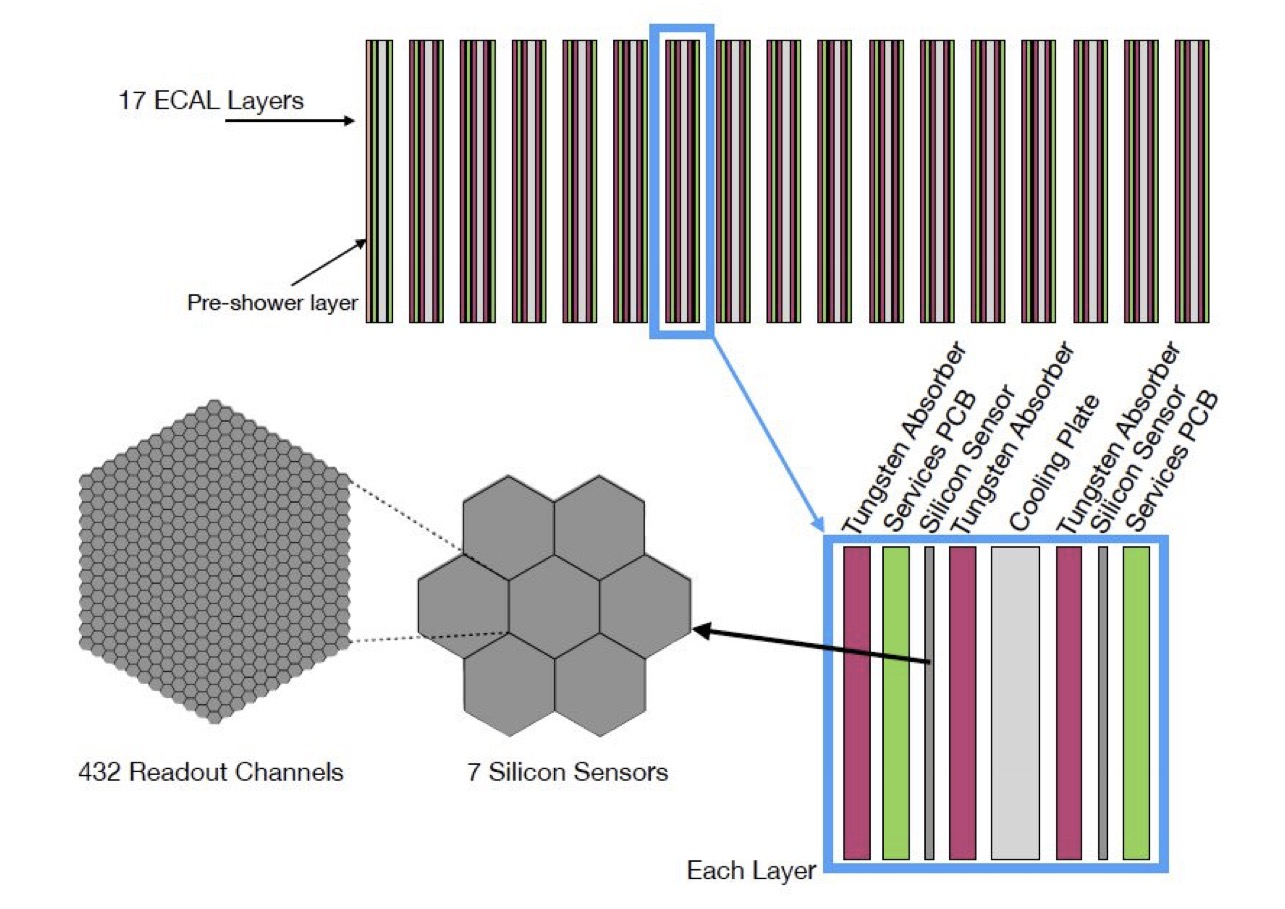
\includegraphics[width=\linewidth]{config/fig/ecal_cells_and_layers.jpg}
    \caption{Schematic of the full-resolution LDMX ECal modules and the
    components of a bilayer. Sourced from the LDMX design report \cite{ldmx2025-overview} }
    \label{fig:ecal_cells_and_layers}
\end{figure}

Each ECal sampling plane contains seven hexagonal modules, and each module
contains 432 silicon readout cells. A local cell identifier connects every
measured energy deposit with a fixed detector position.
Figure~\ref{fig:ecal_cells_and_layers} shows this full-resolution segmentation
and the bilayer construction. For the real-time trigger, groups of nine
neighbouring readout cells are summed into 48 coarser \emph{trigger cells} per
module. This grouping, which is not drawn in the figure, retains less spatial detail for the \textit{online reconstruction} compared to
the individual-cell readout available to \textit{offline reconstruction}
\cite{ldmx2025-overview}.

The fine segmentation helps separate nearby showers and identify small
energy deposits from background particles, making it central to this thesis.
When several beam electrons arrive in the same readout window, their showers
may overlap in the same layers or cells. Reconstruction must then use the
spatial and energy pattern of the full-resolution hits to determine which
electron produced each part of the event and recover per-electron shower
information from the combined response.

\subsubsection{Trigger Scintillator and Trigger-Pad Tracks}

The \gls{ts} estimates how many beam electrons enter the target in the same
readout window and where they pass through the beam region. It consists of
three modules: two directly upstream of the tagging tracker and one directly
upstream of the target. Each module contains two staggered layers of plastic
scintillator bars. A traversing electron deposits energy in a bar and produces
scintillation light that is measured as a photoelectron signal. Adjacent bar
hits are joined into clusters, and clusters across the three modules are
combined when their positions are compatible with an electron travelling
along the expected beam direction \cite{ldmx2025-overview}. Forming these
track candidates is itself a rule-based reconstruction method: low-level bar
signals are converted into estimates of electron position and multiplicity.

In this thesis, the reconstructed TS track candidates are referred to by
their name in the research-group codebase, \texttt{TriggerPadTracks}. The
term describes objects derived from TS measurements, not a separate detector,
and should not be confused as so. Each
candidate provides a one-dimensional position estimate and a photoelectron
count. Together, the candidates provide information about the positions, energy and the 
multiplicity of the incoming electrons. They are reconstructed detector
objects rather than simulation-truth labels, and correspond one-to-one with
the incident electrons only when the reconstruction makes correct prediction \cite{ldmx2025-overview}.

\subsubsection{Triggering
% and reconstruction
}
% I removed the reconstruction from the title since I think that adds reconstruction in too many titles. Reconstruction is already relevant to trigger in itself or maybe one could add a qualitatively description of the trigger that summarizes the content of this section. The trigger naturally leads into online and offline and the different resolutions one works with, and "working" with data is always reconstruction. The term reconstruction should have been defined already before this section I think? 

% We are to refine these section and simplify the description since not all of this information is relevant. Skip the description of trains that does not matter here. 

% One perspective that I have to insert here or in the next section should be that 

% Notes from supervisor: 37,14 MHz bucket, how much in nanoseconds?. beam frequency  kollimerade elektroner först i ett fåtal pikosekunder, sen finns ett 2cmx8cm fönster. 

The beam is divided into short time slots called radio-frequency buckets,
which are delivered in groups called trains. Within a train, neighbouring
buckets are separated by \(26.9\,\mathrm{ns}\), corresponding to a
\(37.14\,\mathrm{MHz}\) clock for the detector electronics. The nominal beam
structure contains 20 filled buckets in each train at a train rate of
\(1\,\mathrm{MHz}\), with an average of approximately one to two electrons
per filled bucket. 
%The estimated frequency of electrons that hit the target is ...??? \textbf{need some input from Lene-Kristian here I think} \cite{ldmx2025-overview}.

Storing the full detector response for every filled bucket is neither feasible nor desirable:
the input rate is much larger than the available readout and storage rate,
and almost all events arise from ordinary processes not displaying the benchmark interaction. 
The online trigger
therefore receives compact information from the \gls{ts}, \gls{ecal} and
\gls{hcal} at the full clock rate and decides in real time whether the complete
event should be read out and stored. The Trigger Scintillator supplies an
incoming-electron count \(n\), and the ECal supplies coarse energy sums. A
basic online estimate is
\begin{equation}
    E_{\mathrm{miss}}^{\mathrm{trig}}
    =
    nE_{\mathrm{beam}} - E_{\mathrm{ECal}}^{\mathrm{trig}} ,
\end{equation}
Here, \(E_{\mathrm{miss}}^{\mathrm{trig}}\) is the trigger-level estimate of
the missing energy, \(n\) is the number of incoming electrons estimated by
the Trigger Scintillator, and \(E_{\mathrm{beam}}\) is the nominal beam energy
per electron. The product \(nE_{\mathrm{beam}}\) therefore estimates the total
incoming energy, while \(E_{\mathrm{ECal}}^{\mathrm{trig}}\) is the energy
measured by the ECal using its coarse trigger readout. The superscript
\(\mathrm{trig}\) distinguishes quantities available to the online trigger
from those obtained through the more detailed offline reconstruction.
Over-counting the electrons can create false missing energy, while
under-counting can cause a real signal event to be rejected. The trigger
reduces the input rate to an average readout rate of about
\(10\,\mathrm{kHz}\). The primary missing-energy trigger uses part of this
bandwidth, while the remainder supports other physics, calibration and
monitoring selections \cite{ldmx2025-overview}.

The distinction between online and offline reconstruction is set by this
decision. Online reconstruction occurs before storage and must satisfy strict
limits on latency, memory and transferred information. It therefore uses
reduced quantities such as ECal trigger-cell sums and Trigger Scintillator
track candidates. Once an accepted event has been fully read out, offline
reconstruction (which techincally has no deadline) can use individual ECal cells and more computationally
demanding algorithms to construct calibrated hits, tracks, showers and
analysis quantities \cite{ldmx2025-overview}.


The methods developed in this thesis use simulated ECal hits at the full cell
granularity, together with reconstructed trigger-pad tracks. They
therefore belong to offline reconstruction research. Their results can show
whether electron showers can be separated under multi-electron conditions.
Deployment in the online trigger would be a separate task because it would
require reduced trigger inputs and a dedicated latency and hardware study.

\subsubsection{Pile-Up, Reconstruction and Physics Reach}
\label{sec:formalism}
% This section is a bit all over the place, it has to be tightened and get a good logical flow. All information that I want to give is contained here it needs to be presented in the best format possibly simply. 

% This section contains too much in one place. It should be broken up where pile-up is one section



% Notes from my supervisor discussion: Multipliciteten beskrivs i en poissonfördelning och den är relativt bred så $\mu = 1$ ger också 2 och 3 elektroner. => det gör att endast $37\%$ av händelserna kan användas







In this thesis, \gls{pile-up} mainly refers to \emph{in-time pile-up}, where
two or more beam electrons arrive in the same time sample and their detector
responses are recorded together. 
\textbf{True?: Trigger latency does not create in-time pile-up. It follows from the number of electrons delivered in the same bucket.}
Lowering the beam intensity would reduce it, but would also
reduce the number of \gls{eot} accumulated per unit time. The practical
challenge is therefore to retain the advantages of higher beam intensity
without losing events because their detector responses are combined
\cite{ldmx2025-overview}.

% The approximation/assumption of independent electron propagation should be mentioned here, but I should also say that one is allowed to this to a very good approximation single electrons are abbysmal low chances of colliding or affecting each other. It is very handy that the eletrons can be approximated as independent since that simplifies computation nicely. 
To a very good approximation, separate beam electrons propagate
independently: the probability that two beam electrons interact directly with
each other is negligible. This simplifies simulation as their propagations 
can be simulated independently and then \emph{overlayed} before simulating their detector responses. Let
\(Z^{(k)}\) denote the true ECal energy-deposition pattern from source
electron \(k\).  Under this simulation assumption,
\begin{equation}
    Z^{(k)} \perp\!\!\!\perp Z^{(\ell)}
    \qquad \text{for } k\neq\ell .
\end{equation}
After overlay and detector reconstruction, the observed hit collection from the detectors is a
combined response,
\begin{equation}
    \mathcal{H}
    =
    \mathcal{R}\!\left(
        Z^{(1)},\ldots,Z^{(m)}
    \right).
\end{equation}
The response \(\mathcal{R}\) is a nondeterministic mapping that includes detector granularity, thresholds,
noise and hit reconstruction. Deposits from different electrons may then
occupy the same cell or form overlapping showers. The observed collection
\(\mathcal{H}\) cannot in general be divided into its original components $Z^{(1)},\ldots,Z^{(m)}$ by
a simple geometric cut.

The overlap affects both triggering and later analysis. An
incorrect electron count can produce an incorrect missing-energy estimate.
Overlapping showers also make the ECal topology harder to interpret and can
cover small deposits that are needed to reject backgrounds. The trigger must
therefore use thresholds that depend on the estimated electron count.
Offline reconstruction can use the full stored detector response to determine
which multi-electron events remain separable and how much per-electron
information can be recovered. Such studies can later inform which event
classes are useful enough to retain at trigger level, although deploying an
online method requires a separate trigger study. This thesis addresses the
offline problem by assigning the combined ECal activity to the different beam
electrons \cite{ldmx2025-overview}.

Multi-electron events are also an opportunity. The design report estimates
that \(4\times10^{14}\) \gls{eot} can be accumulated in about twelve months
with an average of one electron per sample. Reaching exposures of order
\(10^{16}\) \gls{eot} efficiently requires higher beam intensity and the
ability to use events containing several electrons. In a design study with
an average multiplicity \(\mu=1\), accepting up to four reconstructed
Trigger Scintillator tracks instead of only one increased the total signal
trigger efficiency from \(0.58\) to \(0.88\) at approximately the same
\(1\,\mathrm{kHz}\) trigger budget. This result used a
\(0.1\,\mathrm{GeV}\) dark-photon benchmark and the energy in the first 20
ECal layers \cite{ldmx2025-overview}.

% TODO: Add the supervisor's running-time estimate only after the assumed
% beam intensity, target, one-electron selection and personal-communication
% citation have been specified.

Rejecting every multi-electron sample would discard part of the delivered
beam and extend the time needed to reach a given exposure. If overlapping
showers can instead be reconstructed reliably, more recorded events become
useful and the intended sensitivity can be reached sooner. This is how
pile-up handling can increase the practical physics reach of LDMX.

The specific problem studied in this thesis is a step towards that goal. The
study considers two-electron and three-electron events as direct extensions
of the single-electron case; higher multiplicities are outside its scope. The
samples are constructed from independent single-electron simulations, and
the models attempt to assign ECal hits to their electron of origin. The study
does not itself search for \gls{dm}. It tests whether modern reconstruction
methods can recover per-electron shower structure from the combined detector
response produced by multi-electron operation.



\subsection{Machine Learning Methods for Reconstruction in High Energy Physics}
\label{sec:ml_event_reconstruction_hep}


Short introductory text here stating that ML is a topic of rising interest in HEP and refer to output of ML-related papers in HEP. \cite{iml-wg-hepml-livingreview}'. \textbf{I have realized that the relevancy of this section is heavily questioned... Just cherry-pick relevant parts from here and ommit the rest I have limited space and this is not a popular science summary this background should cover necessary theory and it should cover necessary motivation for my study in my thesis, and maybe provide some context for the viewer also but nothing else. The fact that it is a rising tool of interest is still interesting to mention, but only in the contexts of why that is not simply a ''trend follower''. The rising tool of interest should be 1 or max 2 sentences.}


\textbf{text here}

\gls{ml} has become a tool of rising interest in \gls{hep}, driven by the growing complexity of detector data, the need for efficient event selection, and the search for rare signatures of physics beyond the \gls{sm}. At the same time, advances in deep-learning methods and accelerator-based computing architectures such as \glspl{gpu} have made increasingly powerful \gls{ml} and non-\gls{ml} approaches practical for scientific workflows \cite{sur2026-heterogeneous-computing}. Machine learning and deep-learning methods are not new in \gls{hep}, but the recent rapid growth of machine-learning applications in particle physics is 
\begin{wrapfigure}{r}{0.50\textwidth}
    \centering
    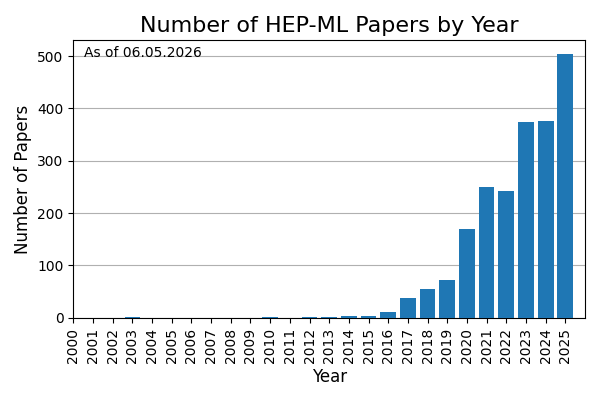
\includegraphics[width=0.48\textwidth]{config/fig/per_year.png}
    \caption{\textbf{Increase the size of labels here} Number of machine-learning-related publications on arXiv in the HEP category per year, based on the Living Review of Machine Learning for Particle Physics \cite{iml-wg-hepml-livingreview}.}
    \label{fig:ml-publications-per-year}
\end{wrapfigure}
reflected both in dedicated reviews and in the continuously updated Living Review of Machine Learning for Particle Physics  \cite{karagiorgi2021-mlnewphysics,feickert2021-livingreview,iml-wg-hepml-livingreview}. Figure \ref{fig:ml-publications-per-year} shows the trend of machine-learning-related publications within \gls{hep} significantly increasing in the last few years. 


The underlying motivation for \gls{ml} in \gls{hep} is that such tools may increase the \textit{physics reach} of experiments, meaning their ability to probe weaker signals, rarer processes, or more challenging regions of parameter space, either by improving sensitivity enabling new discoveries or by making reconstruction and selection more computationally efficient. 

\paragraph{Reconstruction} Reconstruction in \gls{hep} refers to reconstructing the physical interpretables from a measured particle event based on the detector outputs.  Modern \gls{hep} experiments produce high-dimensional and heterogeneous data, where each event may contain a variable number of detector signals distributed across several subdetectors. This makes reconstruction a quite natural application area for machine learning: the task is to transform heterogeneous low-level or intermediate detector information, such as hits, tracks, and calorimeter clusters, into physically meaningful quantities that can be used for triggering, event selection, and analysis.



A useful way to view reconstruction is as an approximate inverse problem. In simulation, a detector may be regarded as a map from an underlying particle-level event to a set of detector measurements. If the particle-level event, representing the physical ''truth'', is denoted by \(Y\), and the corresponding detector response by \(X\), the simulation can be written schematically as
\begin{equation}
    S(Y) = X ,
\end{equation}
where \(S\) represents the detector response. Reconstruction, denoted $R$,  then attempts to inverse the mapping, i.e
\begin{equation}
    R(X) \approx S^{-1}(X) = Y .
\end{equation}
In practice, this inverse is imperfect and often ambiguous, based on the fact that some information is always lost, has stochastic evolutions or only indirectly observed: detector signals have finite resolution and particles may overlap in the detector. These cases does not exclude relevance however, as it could also be useful to study these scenarios as well and infer where our tools of measurement might simply not be enough. Machine-learning-based reconstruction approaches formulate parts of this inverse problem as a learnable mapping from detector-level inputs to physics-level targets, typically using simulated events where truth information is available to us and constructing target information is completely feasible.

\subsubsection{Computational Context in Experimental High Energy Physics}

\textbf{Let Nairit read this section!}

The computational setting of \gls{hep} is also important for understanding the interest in machine-learning-based reconstruction. Large-scale \gls{hep} computing has traditionally been dominated by distributed, \gls{cpu}-based workflows. \cite{sur2026-heterogeneous-computing} This is natural because collision or fixed-target events often are, to a good approximation, independent processes, analog to the electron case of \gls{ldmx} $Z^{(k)} \perp\!\!\!\perp Z^{(\ell)}$ where $k \neq l$, following the notation introduced in Section~\ref{sec:formalism}. Simulation, reconstruction, and analysis can therefore often be parallelized over events with relatively little communication between tasks, making \gls{cpu} clusters and grid computing highly effective, somewhat bypassing an immediate need of software engineering concurrency, which explains the longevity and success of this computing paradigm within \gls{hep}.

At the same time, the wider computing landscape has shifted toward heterogeneous architectures, in particular \glspl{gpu} and other accelerator \footnote{``Accelerator'' in this context refers to specialized hardware such as \glspl{gpu} or even \gls{ml} specialized architectures such as the relatively new \gls{tpu} designed by Google that accelerate the speed of computation for applicable processes\cite{needed}}
-based systems. This development is strongly connected to modern machine learning, where many operations reduce to dense linear algebra and can be executed efficiently on massively parallel hardware, including both training and inference tasks of deep learning \gls{ml} models.

This shift creates both a challenge and an opportunity for \gls{hep}. Rule-based reconstruction algorithms have often been designed around detector-specific logic and sequential or iterative procedures. Such algorithms can be highly effective, but they may be difficult to port efficiently to accelerator hardware and may scale poorly with detector occupancy. Machine-learning models, by contrast, often express reconstruction as a fixed sequence of tensor operations, making inference naturally suited to \glspl{gpu} or other accelerator architectures. 

\subsubsection{MLPF, a Recent Example of ML-based Reconstruction in HEP}

All of the above stated reasons creates a modern context that make up the underlying motivations behind the \gls{mlpf} reconstruction method, designed for the \gls{cms} experiment and the incoming \textit{high luminosity phase} of the \gls{lhc}. The original \gls{mlpf} study published in 2021 used a graph-neural-network-based architecture for efficient particle-flow reconstruction in high-pile-up conditions \cite{pata2021-mlpf}. The latest implementation from early 2026 demonstrates a transformer-based \gls{mlpf} algorithm integrated into the \gls{cms} reconstruction software and evaluated on both simulation and collision data \cite{pata2026-mlpf}. In the latter study, modern hardware, transformer-based computational architectures and recent progress of  the transformer architecture are explicitly part of the motivation for scalable reconstruction in high-dimensional, variable-size event data.

The \gls{mlpf} showcases the motivation for \gls{ml} based reconstruction quite perfectly combining all of the above stated reasons for why \gls{ml} methods have sparked an interest. The \gls{mlpf} uses the modern model architecture, compute is accelerated with modern hardware, the method shows promise of improved speed of compute, resolution of reconstruction and it is motivated by the context of \gls{lhc} high luminosity phase, which will increase complexity with a much higher rate of pile-up.

For the purpose of this thesis, the most relevant role of machine learning is therefore not only as a final classifier that separates signal-like and background-like events, but as a possible reconstruction method. Traditional reconstruction algorithms are often built from physics-motivated rules and detector-specific heuristics. Such methods remain essential, but they may become difficult to optimize in environments with high occupancy, irregular detector geometry, or overlapping detector signatures. Machine-learning-based reconstruction instead attempts to learn parts of the reconstruction mapping $R(X) \approx S^{-1}(X) = Y$ directly from simulated or measured data. It is also important to understand that rule-based and \gls{ml} reconstruction is not either/or, they are the most effective when they work in junction and complement each other. The \gls{mlpf} model takes some object-level inputs that are the results of rule-based reconstruction intermediate outputs such as clusters and particle candidates, in which the \gls{ml}-based \gls{mlpf} can utilize for stronger inference results \cite{pata2021-mlpf}. 

\subsubsection{The GNN and the Transformer under Pile-Up Conditions}

\gls{ml}-based methods are perhaps the most relevant under pile-up conditions, where detector hits from several particles or interactions may overlap and where the association between detector activity and the underlying particle origin becomes ambiguous. In this setting, a model that operates directly on hit-level or object-level detector information may provide additional information beyond a purely rule-based reconstruction, for example by assigning hit-level probabilities or by learning correlations that may be difficult to capture manually with code. One must still remember however that \gls{ml}-methods are certainly also based on ''rules'' in the end, the strength of these methods in this context lie in that their discovery of efficient, or even \textit{optimal} ''rules'', are somewhat automatic and a researcher can explore the space of solutions efficiently.

Architectures such as \glspl{gnn} and \textit{transformer} are particularly well suited to this type of problem because they can operate on variable-size collections of detector objects and learn correlations between them without requiring the data to be arranged on a regular grid. This is important for particle detectors, where the relevant information is often distributed over irregular detector geometries and across multiple subdetectors. By contrast, architectures such as \glspl{cnn} are naturally adapted to regularly spaced image-like data and therefore impose an inductive bias that is not always well matched to detector readout. Graph-based models instead allow calorimeter hits, clusters, tracks, or other detector objects to be represented as nodes, with edges describing geometrical proximity or learned relationships. Transformers provide a related approach but it uses different analogies than nodes and edges. 

In this thesis, the same general motivation is applied to the \gls{ldmx} setting. The aim is not to perform full general-purpose particle-flow reconstruction, as in \gls{cms}, but to build and study a reconstruction platform for identifying electron-induced activity in the electromagnetic calorimeter down to hit-level statistics, especially under pile-up conditions. This is the regime where reconstruction ambiguities are expected to be most relevant, and where machine-learning methods may offer the largest benefit over rule-based approaches.

\textbf{This is kind of outdated, should I include all of this or not?} The rest of this subsection introduces the machine-learning context needed for the reconstruction study in this thesis. First, the existing rule-based reconstruction chain in \gls{ldmx} is reviewed, with emphasis on clustering, particle-flow-inspired reconstruction, and the distinction between online and offline reconstruction. The existing machine-learning-based veto strategy in \gls{ldmx} is then briefly discussed, since it represents an already planned use of machine learning in the experiment \textbf{not relevant for my study?}. The subsection then turns to machine-learning-based reconstruction in \gls{cms}, in particular the development of \gls{mlpf}, which provides a useful point of comparison for the approach studied here. Finally, the basic ideas behind \glspl{gnn} and transformers are introduced and compared. These architectures form the methodological basis for representing calorimeter hits and other detector objects as unordered sets of nodes or tokens, allowing event reconstruction to be formulated as a learnable mapping from detector-level inputs to physics-level targets.

\textbf{Further motivation of why not to use CNN to use somewhere maybe:}

This representation preserves individual detector objects rather than
projecting the event to an image. The number of hits is event dependent, the
\gls{ecal} is 3D, and overlapping showers need not be aligned
with a fixed rasterization. Moreover, trigger-pad-track information is not an
\gls{ecal} pixel quantity. Sets, learned graphs and attention-based token
sequences provide natural ways of relating these heterogeneous objects while
remaining insensitive to an arbitrary ordering of the input rows.

\subsubsection{Graph Neural Networks and GravNet}
\label{sec:gnn_gravnet_background}

A graph represents a collection of objects as nodes and specifies which pairs
of nodes are connected by edges. Applied for \gls{hep} in reconstruction, a node can
represent information from a subdetector: a calorimeter hit, a track or another detector object (some detector-derived quantity, for example computed clusters), with its
measured quantities stored in a feature vector \(\mathbf{x}_i\) as input. The edges
define which nodes may exchange information. This makes graphs suitable for
variable-size data on irregular detector geometries, without assigning a
physical meaning to the order in which the objects are stored, which may seem like a interesting proposition for a physicist in \gls{hep} explaining their rising popularity in this field
\cite{duarte2020-gnn-tracking}.

In the message-passing formulation used here, each layer first constructs a
message from every neighbour \(j\) of node \(i\). The incoming messages are
combined and used to update the representation of node \(i\):
\begin{equation}
    \mathbf{a}_i^{(\ell)}
    =
    \underset{j\in\mathcal{N}(i)}{\operatorname{AGG}}
    M^{(\ell)}
    \!\left(
        \mathbf{h}_i^{(\ell)},
        \mathbf{h}_j^{(\ell)}
    \right),
    \qquad
    \mathbf{h}_i^{(\ell+1)}
    =
    U^{(\ell)}
    \!\left(\mathbf{h}_i^{(\ell)},\mathbf{a}_i^{(\ell)}\right).
    \label{eq:generic_message_passing}
\end{equation}
Here, \(M^{(\ell)}\) and \(U^{(\ell)}\) are learned functions and
\(\operatorname{AGG}\) is an order-independent operation such as a sum,
mean or maximum. The updated feature therefore depends on the node itself and
on information received from its neighbourhood. Stacking layers allows
information to travel farther through the graph
\cite{gilmer2017-message-passing,duarte2020-gnn-tracking}.

\glsunset{gravnet}
The \gls{gravnet} layer is a message-passing layer in which the graph itself
is learned. From every current node representation \(\mathbf{h}_i\), two
linear projections produce coordinates \(\mathbf{s}_i\) in a learned space
and features \(\mathbf{f}_i\) to propagate. The coordinates are not physical
positions, although physical detector coordinates may be included among the
input features. Each node is connected to its \(k\) nearest neighbours in the
learned space. Its messages can be summarized as
\begin{align}
    \mathbf{s}_i &= \mathbf{W}_s\mathbf{h}_i+\mathbf{b}_s,
    &
    \mathbf{f}_i &= \mathbf{W}_f\mathbf{h}_i+\mathbf{b}_f,
    \nonumber\\
    \mathbf{m}_{j\rightarrow i}
    &=
    \exp\!\left(
        -c\left\lVert\mathbf{s}_i-\mathbf{s}_j\right\rVert_2^2
    \right)\mathbf{f}_j,
    &
    j&\in\mathcal{N}_k(i),
    \label{eq:gravnet_message}
\end{align}
where \(c>0\) is a fixed distance scale and where............ Nearby nodes in the learned space
therefore contribute more strongly. The \texttt{GravNetConv} operation takes
the element-wise mean and maximum of these messages and combines both with a
transformed version of the original node feature to produce
\(\mathbf{h}'_i\). A new neighbourhood is constructed in every GravNet layer,
so the relations between detector objects can change as their representations
develop. Figure~\ref{fig:gravnet_convolution} summarizes this sequence of
operations \cite{qasim2019-gravnet}.


\textbf{Flowchart here? Good to include or not visualizing GNN or the gravnetconv specifically?
}

The models in this thesis use either \gls{ecal} hits alone or \gls{ecal} hits
and trigger-pad-track observations as nodes. A stack of
\texttt{GravNetConv} layers returns one representation per input node. A
shared output head produces one prediction vector per node, after which only
the predictions for \gls{ecal} hits are retained for the hit-origin task. The
exact input features and model configuration are specified in
Sections~\ref{sec:method_features} and~\ref{sec:method_models}, respectively.

\subsubsection{Transformer Encoders and Self-Attention}
\label{sec:transformer_encoder_background}

A Transformer operates on input objects called \emph{tokens}. A token need
not represent a word. In this thesis, tokens represent selected \gls{ecal}
hits and, in the mixed-detector models, trigger-pad-track observations. A
shared input network maps the feature vector \(\mathbf{x}_i\) of each token to
a latent representation \(\mathbf{h}_i\in\mathbb{R}^{d_{\mathrm{model}}}\).
For an event containing \(n\) tokens, these representations form a matrix
\(\mathbf{H}\in\mathbb{R}^{n\times d_{\mathrm{model}}}\).

The central operation of a Transformer encoder is \emph{self-attention}. For
one attention head, three learned linear projections produce a query, key and
value for every token:
\begin{equation}
    \mathbf{Q}=\mathbf{H}\mathbf{W}_Q,
    \qquad
    \mathbf{K}=\mathbf{H}\mathbf{W}_K,
    \qquad
    \mathbf{V}=\mathbf{H}\mathbf{W}_V.
    \label{eq:transformer_qkv}
\end{equation}
The projection matrices \(\mathbf{W}_Q\), \(\mathbf{W}_K\) and
\(\mathbf{W}_V\) are learned during
training. The queries, keys and values themselves depend on the input event.
Scaled dot-product attention is then
\begin{equation}
    \operatorname{Attention}(\mathbf{Q},\mathbf{K},\mathbf{V})
    =
    \operatorname{softmax}
    \!\left(
        \frac{\mathbf{Q}\mathbf{K}^{\mathsf{T}}}{\sqrt{d_k}}
    \right)
    \mathbf{V},
    \label{eq:scaled_dot_product_attention}
\end{equation}
where \(d_k\) is the query and key dimension and the softmax is applied to
each row \cite{vaswani2017attention}. The query of token \(i\) is compared
with the key of every token \(j\). The resulting weight determines how much
of the value \(\mathbf{v}_j\) contributes to the updated representation of
token \(i\). Full self-attention therefore lets every detector object in an
event receive information directly from every other object.

A multi-head attention layer repeats this operation with separate sets of
projections. The head outputs are concatenated and projected, which allows
different heads to learn different token-to-token relations. An encoder layer
then applies the same two-layer feed-forward network, with a ReLU activation,
independently to each token. Residual connections and layer normalization are
used around both the attention and feed-forward operations, and several
encoder layers can be stacked. One encoder layer is summarized in
Figure~\ref{fig:transformer_encoder} \cite{vaswani2017attention}.

\textbf{Figure here? Good to include or not visualizing GNN or the gravnetconv specifically?}




The original Transformer adds a positional encoding because word order is
meaningful. The row order of detector objects has no corresponding physical
meaning, so the encoder models used in this thesis do not encode the arbitrary
row index. Physical position is instead supplied through detector-coordinate
features. Without a row-position encoding, self-attention is permutation
equivariant: reordering the tokens produces the same reordering of the
per-token outputs \cite{lee2019-set-transformer}. Shorter events are padded
when events are batched, and a mask prevents real tokens from attending to the
padded rows.

The models in this thesis use only the Transformer encoder, not the
autoregressive decoder of the original architecture. The encoder returns one
representation per token. Task-specific heads use these representations for
per-hit predictions, while pooled representations can also support event-level
predictions. Each attention head forms an \(n\times n\) matrix of pairwise
weights, so the memory and computational cost of full attention grow
quadratically with the number of tokens. Its global information exchange also
provides the connection to graph message passing developed in the next
subsubsection.


\subsubsection{An analogy between the Transformer and the GNN}

% What is this complexity? Is it approximate parameter count given input N? Does that correspond to the internal representation as well that could be interpreted as a graph as well for a transformer as for a gravnet? I think this perspective might be interesting to include in this section that highlights the differences and similarities between transformer and gnns. 
Transformer $(O(N^2))$ 
Gravnet $(O(Nk))$


The Transformer is a special case of a \gls{gnn}. This analogy is relevant to be aware of, and the name \gls{gnn} refers rather to a large catalogue of different implementations but what they all have in common that the input has a suitable analogy as being seen as nodes in a graph in the learned representation of the network, and then message passing is performed along these. The input to a transformer are called tokens, or even sloppily called words in the context of natural language processing, but one can mathematically show how a generic \gls{gnn} could be molded into an equivalent network of a transformer, something Chaitanya K. Joshi has derived \cite{joshi2025transformersgnn}, adding to deconstructing the distinction around the terms nodes and tokens. 

There is also another \gls{gnn} architecture that is kind of the middle ground of a generic \gls{gnn} and the transformer, known as \gls{gat}, which implements the attention mechanism to \gls{gnn}s, but the attention is not applied globally and being still restricted to local neighborhoods. The derivation in Joshi's paper molds a \gls{gnn} into a transformer by considering a \gls{gnn} with a fully connected graph (i.e, global) and also implementing the attention mechanism to it, obtaining a mathematical equivalent between the two networks \cite{joshi2025transformersgnn}. 

The architectural differences between the two networks might have been blurred, but the transformer architecture has one benefit over the \gls{gnn} currently, namely of \textit{''winning the hardware lottery''} \footnote{The term, introduced by Sara Hooker, describe when a
research idea in computer science wins because it was suited to the available software and hardware and not because the idea is superior to alternative research directions. \cite{hooker2020hardwarelottery}}. There is one practical difference between the two classes, and that is that 
the self-attention mechanism for all tokens in
an input set $\mathscr{S}$ can be computed in a highly parallelized manner as follows:

\[
\widetilde{\mathbf{H}}^{\ell}
=
\operatorname{softmax}
\left(
\mathbf{H}^{\ell}{W}_{Q}^{\ell}
\left(
\mathbf{H}^{\ell}{W}_{K}^{\ell}
\right)^{\top}
\right)
\left(
\mathbf{H}^{\ell}{W}_{V}^{\ell}
\right).
\]

Where $\mathbf{H} \in \mathbb{R}^{n \times d}$ is a matrix of initial representations. 
\textbf{(i took these snippets directly and I dont know how much I want to include or how I can condense)} 
\textbf{snippet 1:} Transformers implement global multi-head attention through highly optimized dense matrix multiplication operations that leverage the parallel processing capabilities of modern \gls{gpu}s and \gls{tpu}s. \cite{joshi2025transformersgnn}.
\textbf{snippet 2:} The multi-head attention mechanism can also be similarly parallelized by performing a single linear
transformation for all heads in parallel, followed by reshaping the queries, keys, and values per head
to tensors of dimension n×k×d/k each. The token-wise operations which follow multi-head
attention are independent of other tokens and trivially parallelizable as well.
In contrast, GNNs typically perform sparse message passing over locally connected structures, which
is substantially less efficient on current GPUs for typical problem scales (with the exception of very
sparse or billion-scale graphs). This involves maintaining an index of neighbours for each node,
and performing gather and scatter operations to propogate messages [Fey and Lenssen, 2019]. As a
result, GNNs are orders of magnitude slower to train and challenging to scale compared to standard
Transformers on current hardware.

\textbf{My text again:} This means that if one would design one \gls{gnn}-based model and one transformer-based model whose performance on their tasks are equally accurate, then the transformer-based model is, if no other apparent downsides, likely the better choice since inference and training will run faster and more efficient on the modern hardware, at least given the clear current shift in the hardware industry. The speed of inference is also especially important if one would design a \gls{ml}-based online reconstruction model meant for being used, at some capacity, in real-time of the experiment, maybe even in triggering. The aspect of speed on modern hardware is specifically one of the mentioned reasons for why the latest iteration of the \gls{mlpf} model abandoned \gls{gnn}s for transformers instead \cite{pata2026-mlpf}. 



%\textbf{Self critical question and reminder:} How does this subsubsection relate to my thesis?

%\textbf{answers:} Becuase it is a valuable lesson for the reader navigating in this landscape trying to represent detector data as nodes/tokens to know that they are almost exactly the same thing if we look at the transformer! It explains why transformers are interesting as well, since GNNs have had a previously established relevancy in ML HEP, thus transformers are an alternative that should perform quite well. In this analogy context, we should also consider the practical benefits of using a transformer architecture. Hardware is currently being designed for the transformer architecture specifically, thus there are computational benefits of sticking with the transformer architecture instead of relying on message parsing computations of the gnn. This leads to the practical "lemma" that if I would find in my analysis that the models perform equally well in accuracy, then I would recommend the transformer model, which is a very practical and sensible conclusion that I can refer back to! This explains why tokens/nodes are essentially the same. It explains the hardware lottery term it can be resused in discussion. 

%\textbf{Starting Ideas:} The transformer and the gnn architectures are distinct architectures but they also have similarities and one can mold the gnn to essentially become a transformer: there exist an analogy between them and I believe it is revolved around a fully connected graph gnn is essentially a transformer (but without the self attention mechanism?) and vice versa. Explain how a fully connected graph can be compared to a transformer. Explain a transformer and explain the attention mechanism. What is the stepping stone distance going from a GNN to a transformer? Why could that be reasonable? Does it anticipate to introduce new challenges?

%\textbf{comments: explain the attention mechanism should possibly be made earlier? then the reader already understand the math used above}

%*Figure somewhere illustrating the idea of GNN in HEP reconstruction and subdetector data (probably omit if there is a proper one later anyways)*


\subsection{things that I want to include but have not found a suitable place yet}

Briefly mention clustering and reconstruction methods that LDMX has already implemented and plans to potentially use. Describe these existing LDMX reconstruction approaches very shortly, and these are based on other methods developed at CMS CERN already (clustering CLUE, particle flow PF), where the the detector design such as the ECal is the inspiration and what LDMX is based at giving that the LDMX detector is a so-called "sibling detector".

Briefly mention that machine learning approaches have been explored by previous thesis students testing CNN, GNN and even RNN, and reference these.

Briefly mention and explain and a particle-net (GNN) implementation that was made for ML-based Veto in LDMX (explain what a veto is).


\subsubsection{ML-based Reconstruction in CMS}

\textbf{comment: This is a title that I think was interesting when I thought to explain particlenet, though I have come to the conclusion with my supervisor that explaining and detailing other reconstruction methods is not directly relevant to my work and there is not enough time to expand my analysis or to explain all of this in detail I can only briefly mention it for useful context for the reader and to motivate my study compared to previous students.}


%Beyond physics performance, the \gls{mlpf} studies are relevant because they connect reconstruction algorithms to modern heterogeneous computing. The original graph-based \gls{mlpf} work emphasized scalable graph construction and accelerator-friendly inference \cite{pata2021-mlpf}, while the later \gls{cms} implementation demonstrated that a transformer-based reconstruction model can be integrated into the \gls{cms} software framework and evaluated on \gls{gpu} hardware \cite{pata2026-mlpf}. This makes \gls{mlpf} an example not only of machine-learning-based reconstruction, but also of how reconstruction algorithms may adapt to the changing computational architecture of \gls{hep}.
